\begin{center}
    \thispagestyle{empty}
    \vspace*{\fill}
    \textbf{\large Team Pegasus}\\
    % add logo
    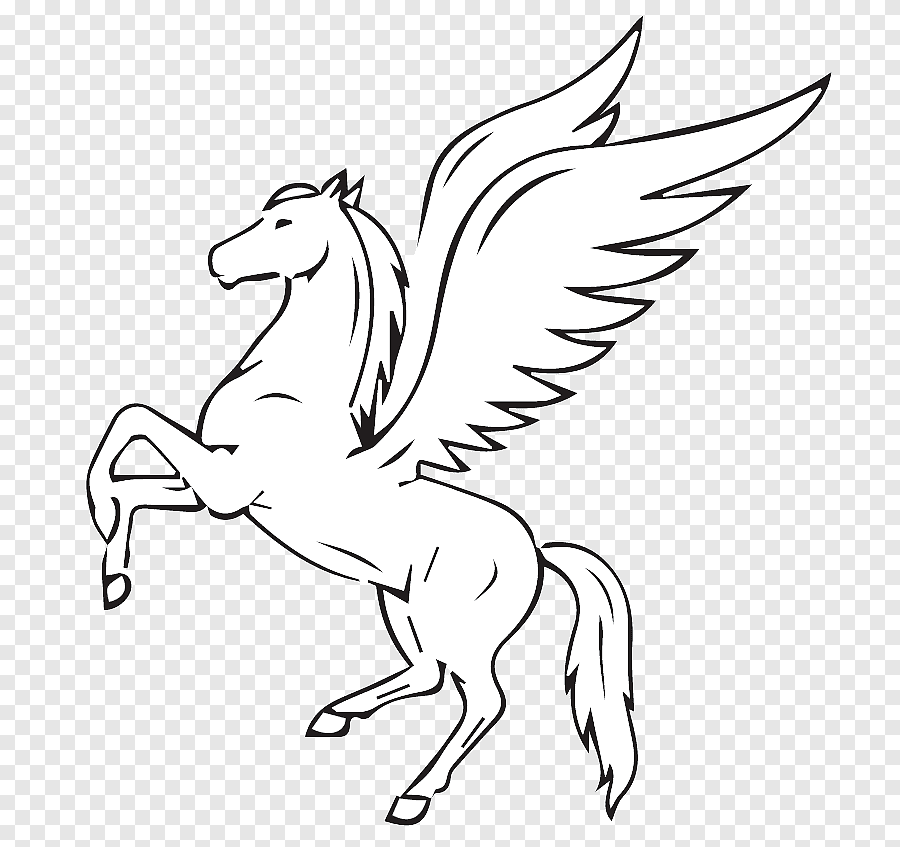
\includegraphics[width=0.35\textwidth]{img/pegasus.png}\\
    \vspace*{\fill}
    \abstract{
        \noindent
        \begin{flushleft}
        The study presented in this paper explores the dynamics of predictive language processing through the visual world paradigm (VWP), a widely employed method in cognitive psychology. The primary objective of the research is to unwind how individuals anticipate or predict forthcoming words during the unfolding of the spoken instructions. The Gazepoint GP3 eye tracker is leveraged for precise gaze pattern analysis. The investigation delves into the impact of competitor words on gaze patterns, to study the cognitive mechanisms underlying real-time language comprehension. Our experiment uses a collection of competitor words sharing phonetic or semantic similarities with the target, and validates the hypothesis that the existence of such competitors leads to an increased number of fixations on them, reflecting the participants' evolving predictions of the upcoming word.
        \end{flushleft}
    }
\end{center}